\documentclass[11pt]{article}
\usepackage[utf8]{inputenc}
\usepackage{amsmath, amssymb, graphicx, subcaption, tabularx, booktabs}
\usepackage[numbers]{natbib}
\usepackage{glossaries}
\makeglossaries

% Comprehensive preamble for compatibility
\usepackage{geometry}
\geometry{a4paper, margin=1in}
\usepackage{times}
\usepackage{parskip}
\usepackage{tikz}
\usetikzlibrary{shapes.geometric, arrows.meta}

% Font configuration (last in preamble)
\usepackage[T1]{fontenc}
\usepackage{mathptmx}

% Glossary entries
\newglossaryentry{Decelerationism}{name=Decelerationism, description={A governance framework slowing platform-driven entropy and rewarding semantic novelty, critiquing accelerationism and effective accelerationism (e/acc).}}
\newglossaryentry{e/acc}{name=e/acc, description={Effective accelerationism, advocating rapid AI scaling, countered by Decelerationism’s compression focus.}}

\title{The Vanity Press Economy: From Patronage to Platform Enclosure}
\author{Anonymous}
\date{October 2025}

\begin{document}
\maketitle

\begin{abstract}
This essay examines the evolution of knowledge economies from seventeenth-century royal vanity presses to modern AI-driven platforms, proposing \gls{Decelerationism} to counter entropic acceleration. Initially termed ``Deccelerationism'' to highlight compression and critique \gls{e/acc}, \gls{Decelerationism} slows platform capture via a Compression Commons and transparency mechanisms, rewarding novelty (\(\Delta K\)) and penalizing redundancy.
\end{abstract}

\section{Introduction}
The vanity press economy, from royal patronage to platform feudalism, amplifies entropy while capturing user-generated novelty. \gls{Decelerationism}, adopted for clarity, critiques accelerationism and \gls{e/acc} \citep{BasedBeffJezos2023}, proposing governance to preserve agency and semantic value (Sections \ref{sec:compression}, \ref{sec:commons}).

\section{From Royal Patronage to Web 2.0}
\label{sec:history}
Royal vanity presses (1600s) subsidized knowledge via prestige \citep{Biagioli2002}. By 2010, platforms inverted subsidies (\(\sigma(t)\)), extracting user value (Figure \ref{fig:subsidy}).

\begin{figure}[h]
\centering
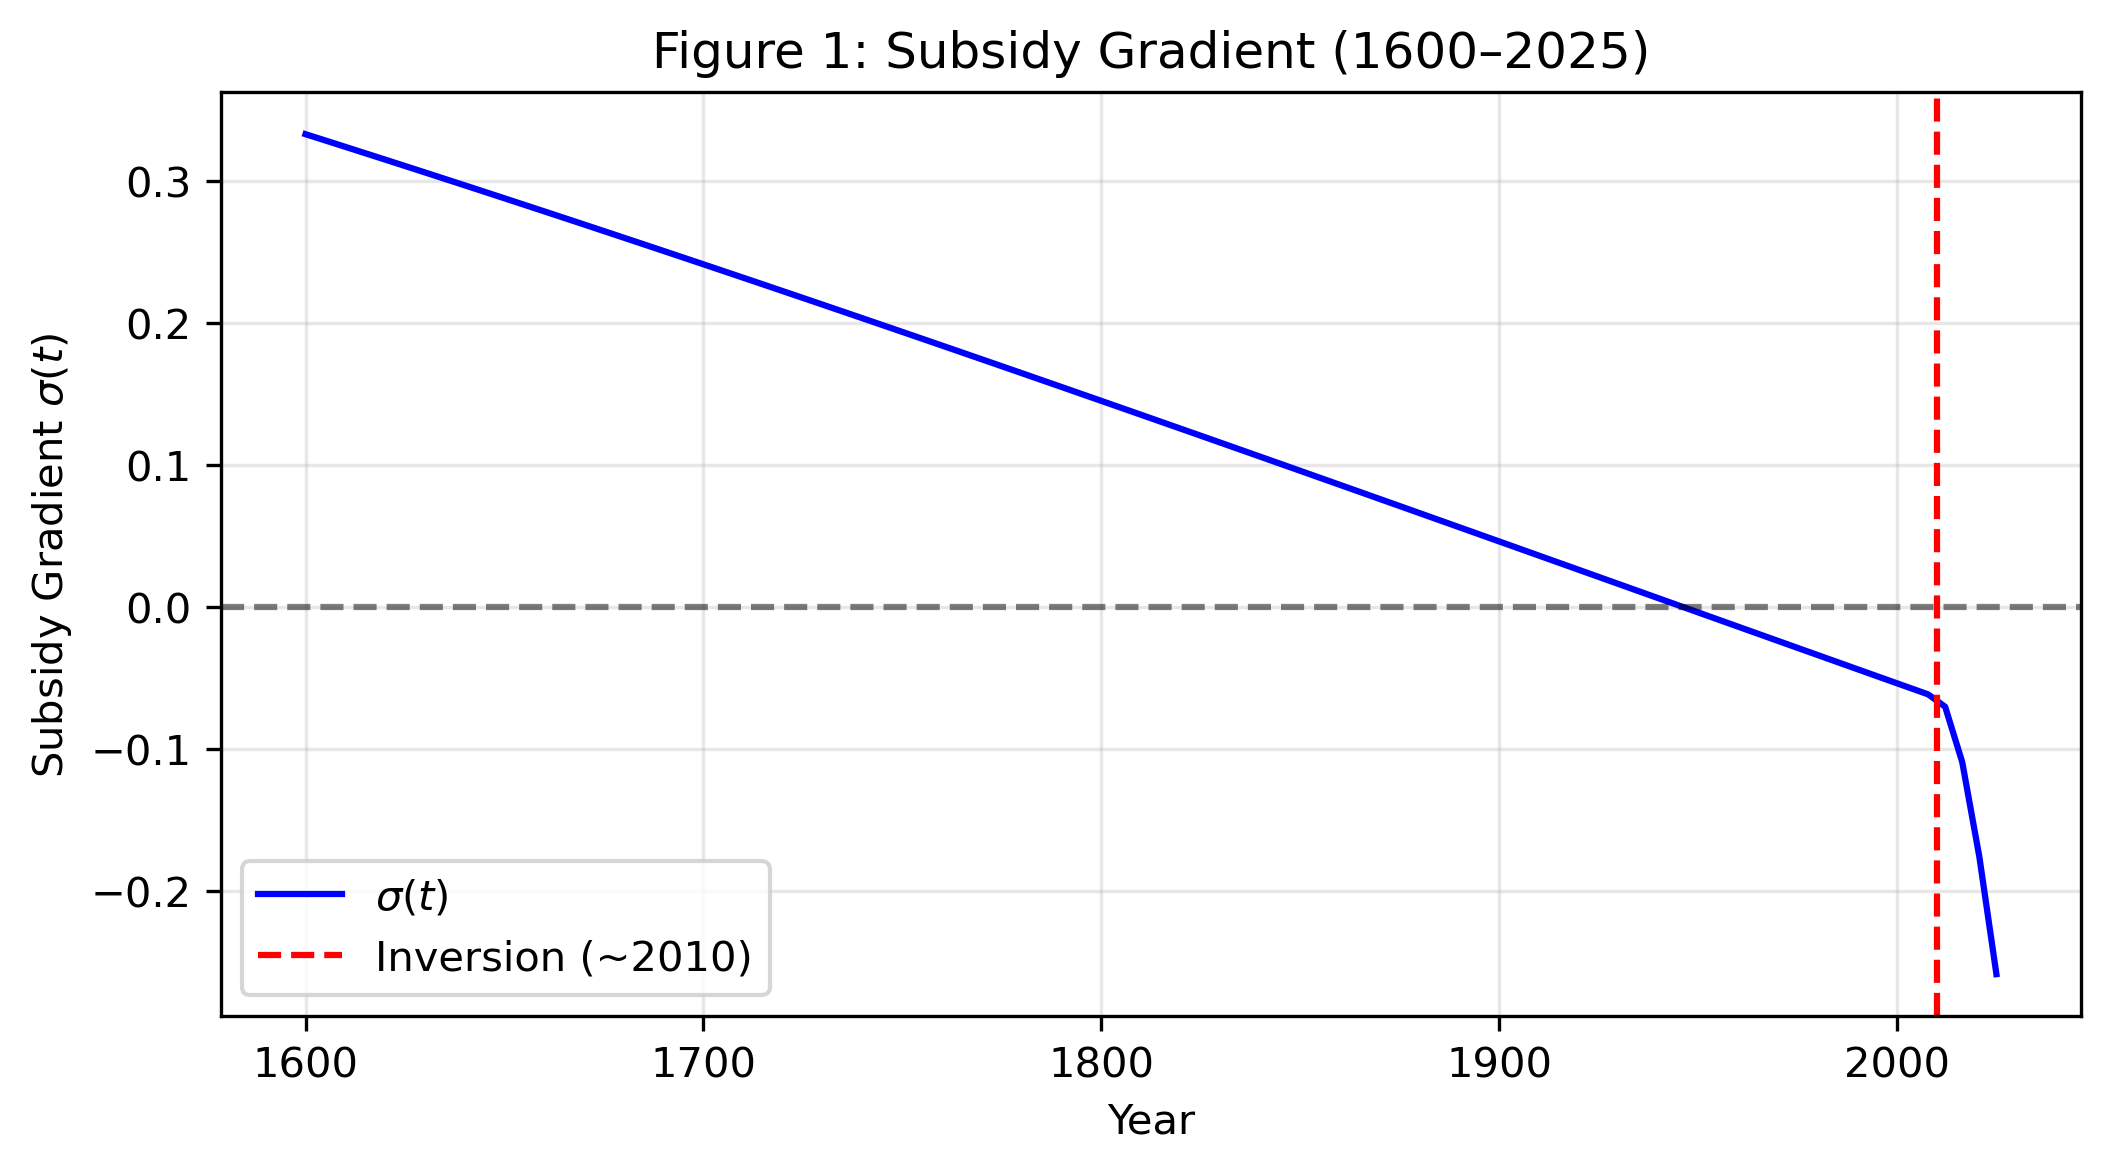
\includegraphics[width=0.5\textwidth]{figures/subsidy_gradient.png}
\caption{Subsidy Gradient $\sigma(t)$: Transition from Patronage to Enclosure (1600–2025).}
\label{fig:subsidy}
\end{figure}

\section{RSVP Dynamics}
\label{sec:rsvp}
Platform attention flows follow RSVP equations (Appendix B), visualized in Figure \ref{fig:rsvp}.

\begin{figure}[h]
\centering
\begin{subfigure}{0.45\textwidth}
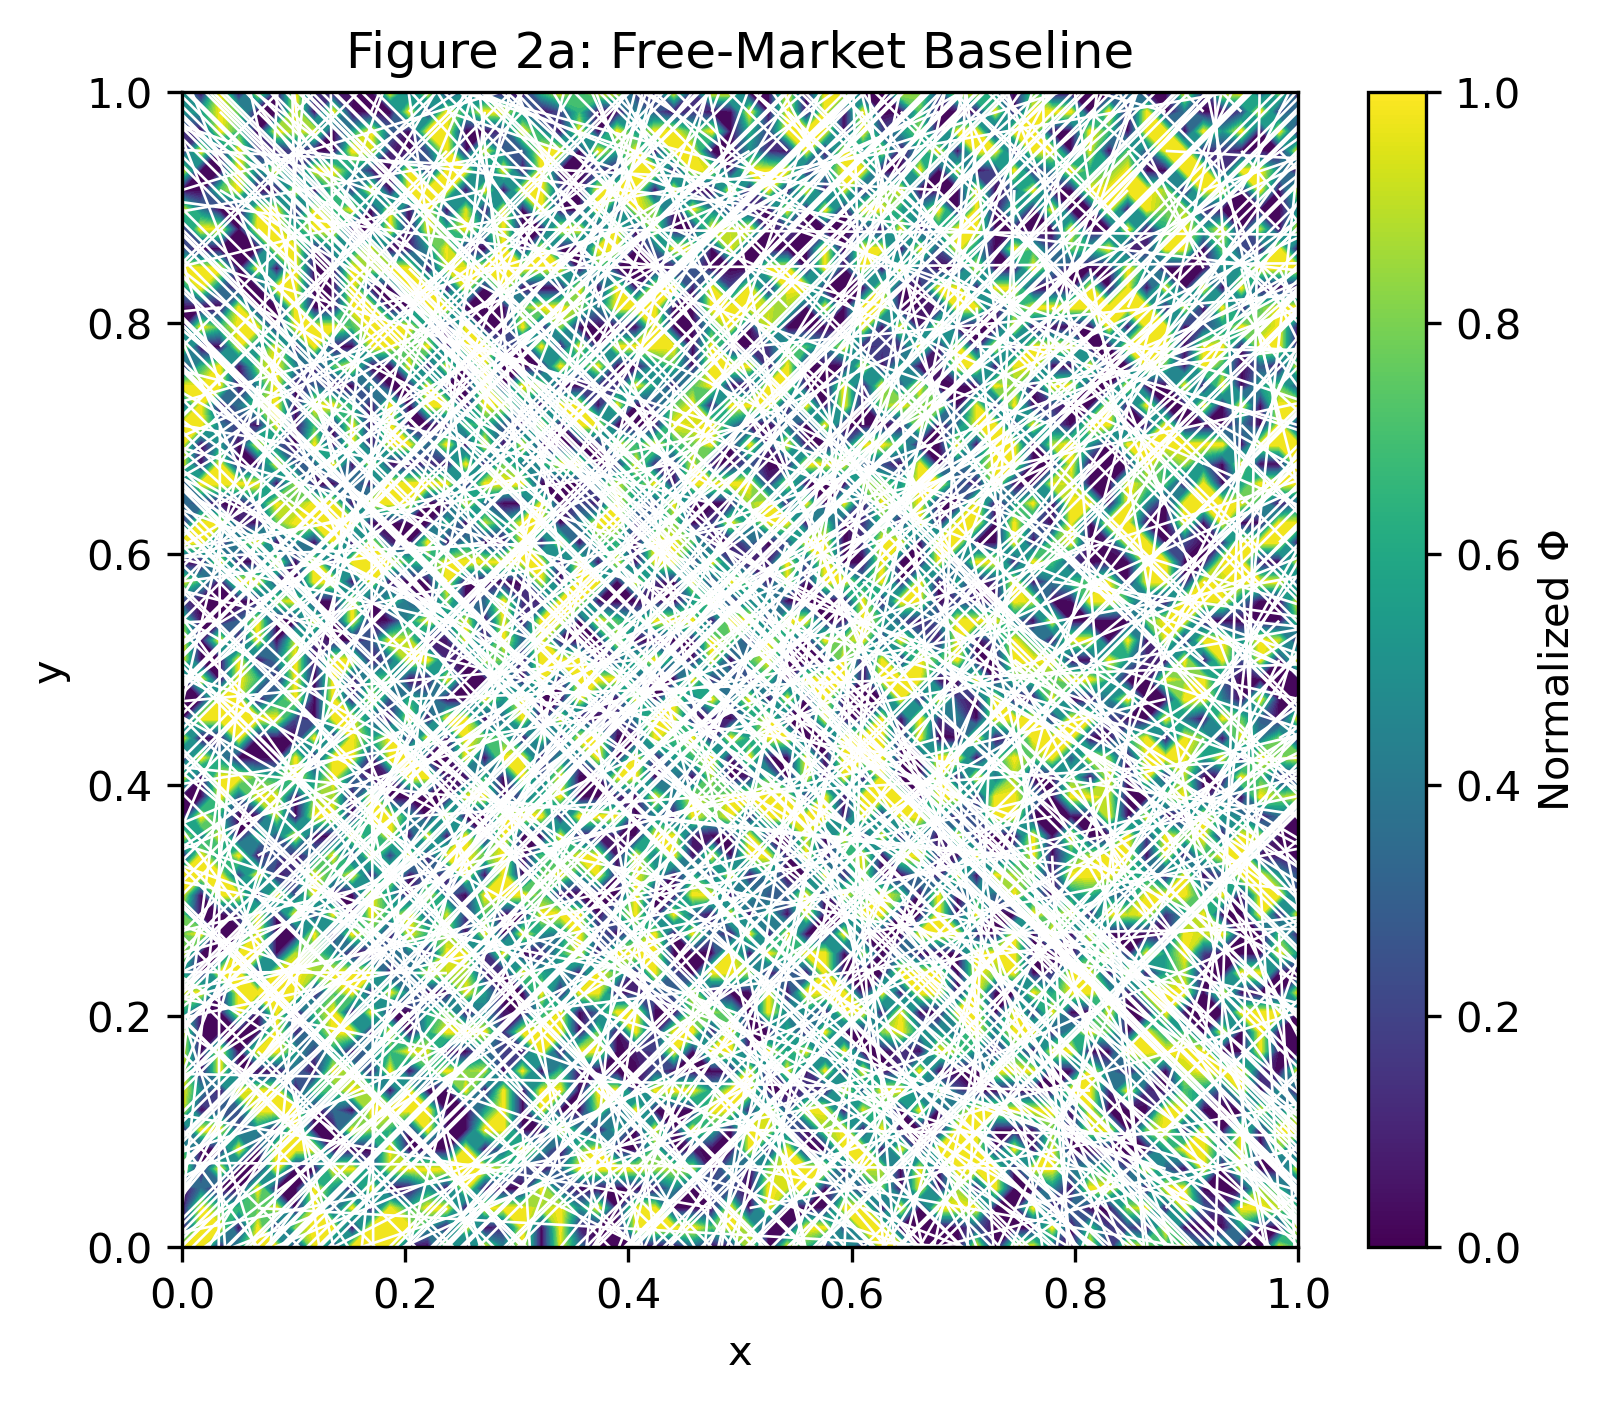
\includegraphics[width=\textwidth]{figures/rsvp_free.png}
\caption{Free-Market Baseline}
\label{fig:rsvp_free}
\end{subfigure}
\hfill
\begin{subfigure}{0.45\textwidth}
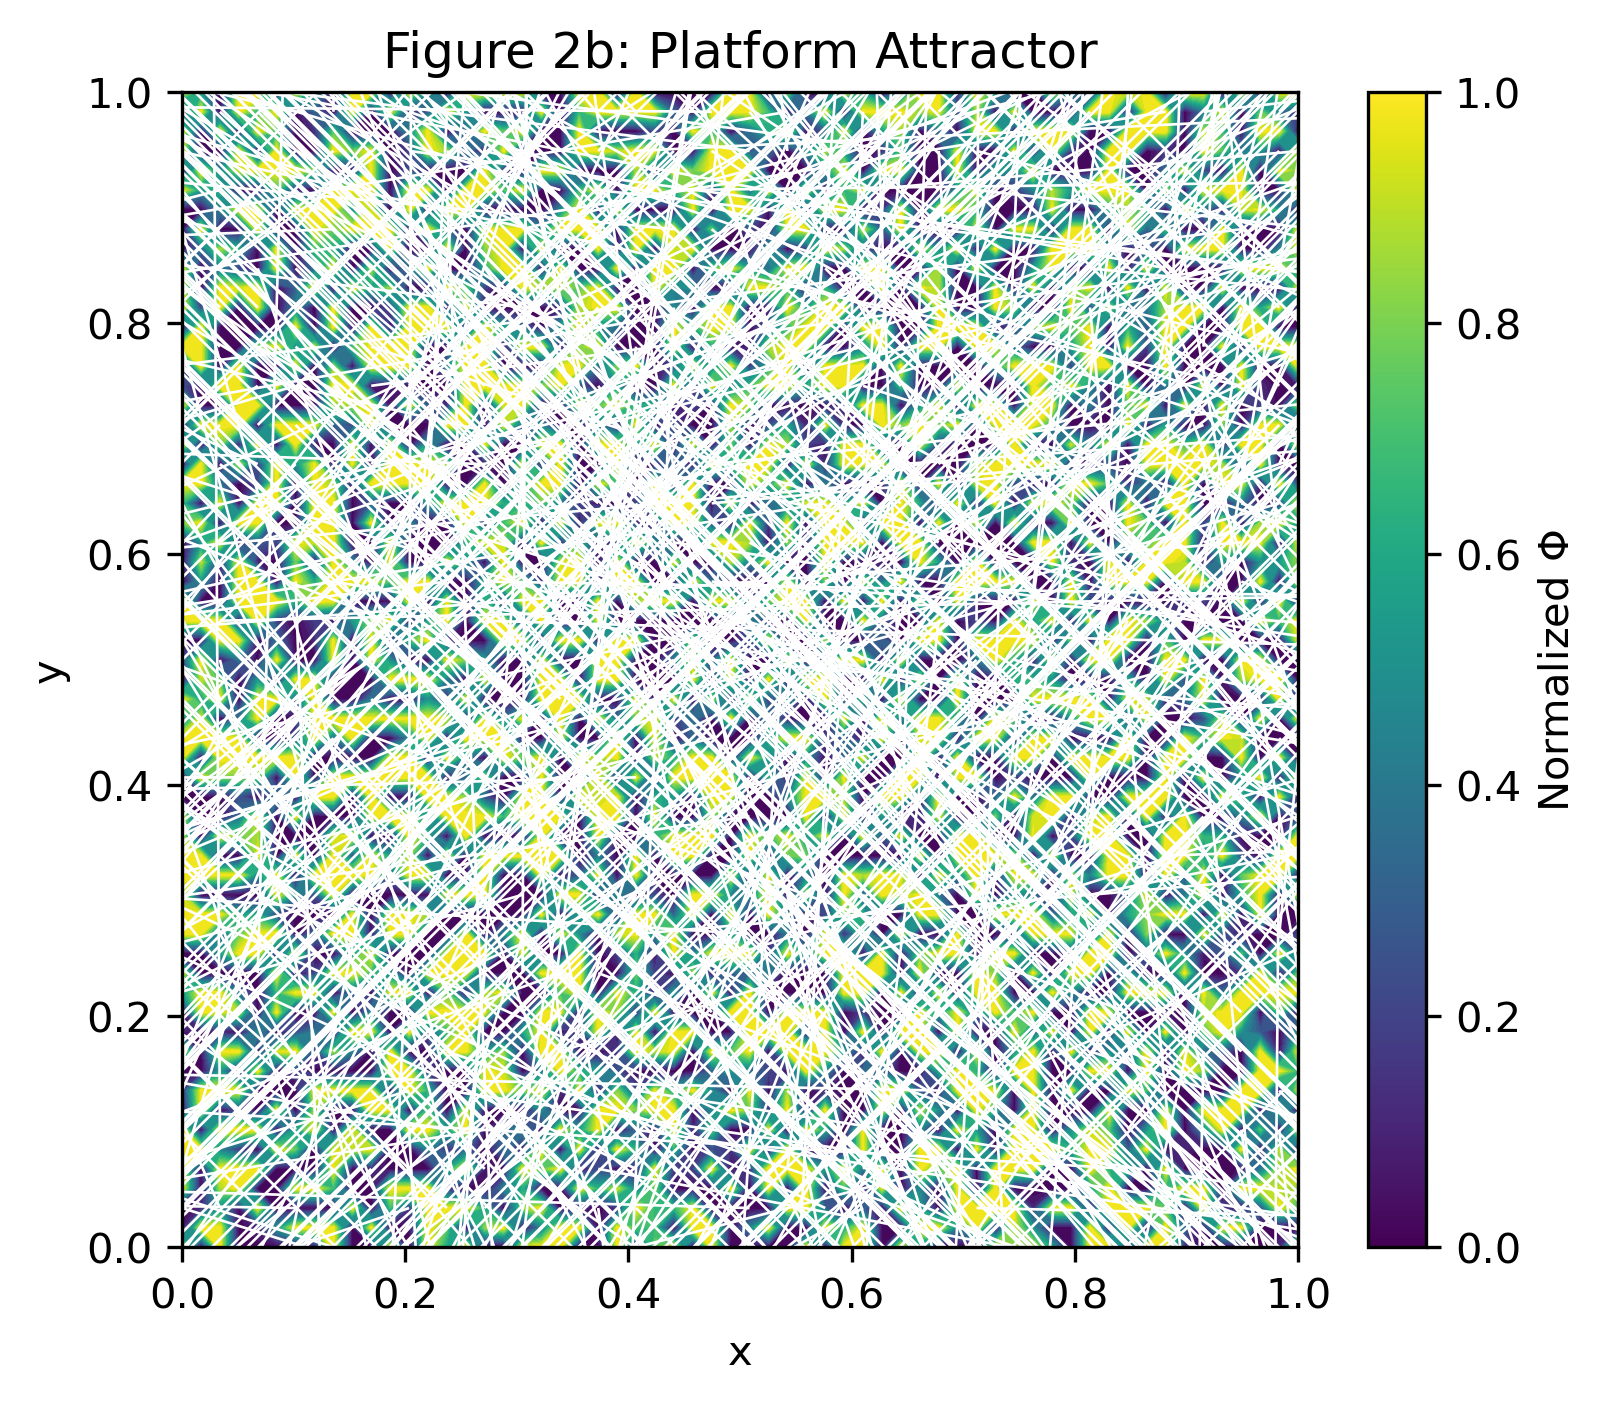
\includegraphics[width=\textwidth]{figures/rsvp_attractor.png}
\caption{Platform Attractor}
\label{fig:rsvp_attractor}
\end{subfigure}
\caption{RSVP Phase Portraits: Distributed vs. Attractor Regimes.}
\label{fig:rsvp}
\end{figure}

\section{Compression Economics}
\label{sec:compression}
Compression progress (\(G \approx \log P_{\text{old}} - \log P_{\text{new}}\)) measures novelty \citep{Schmidhuber2009}, but platforms capture \(\Delta K\) (Figure \ref{fig:compression}).

\begin{figure}[h]
\centering
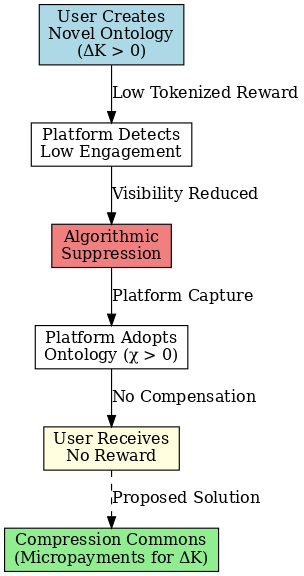
\includegraphics[width=0.5\textwidth]{figures/compression_theft.png}
\caption{Compression Theft Flowchart: From User Innovation to Platform Capture.}
\label{fig:compression}
\end{figure}

\section{Compression Commons}
\label{sec:commons}
The Compression Commons redistributes \(\Delta K\) via micropayments, countering \gls{e/acc}’s scaling dogma.

\section{Transparency and Sousveillance}
\gls{Decelerationism} extends Brin’s sousveillance \citep{Brin1998} to expose platform opacity, reducing \(\chi = \Delta K_{\text{captured}} / \Delta K_{\text{created}}\).

\section{Nine Directives}
\begin{table}[h]
\caption{Nine Directives Mapping}
\begin{center}
\begin{tabular}{lcc}
\toprule
Directive & Pathology & Remedy \\
\midrule
Withhold Strategically & Subsidy Inversion & $\text{Hom}(X,Y) \setminus W$ \\
Diffuse Redundancy & e/acc Scaling & Decentralized nodes \\
\bottomrule
\end{tabular}
\end{center}
\label{tab:directives}
\end{table}

\appendix
\section{RSVP Simulation}
Parameters: \(\lambda_{\Phi S} = 0.1\), \(\eta_{vS} = 0.02\), \(\alpha = 1.0\), \(\beta = 0.2\), \(\gamma = 0.05\).

\section{Pilot Data}
Pilot estimates: \(\widehat{\lambda}_{\Phi S} = 0.12 \pm 0.02\)/day (Wikipedia, January 2025).

\section{Conjectures}
\textbf{D.1 Rent Bound.} Conjecture: \(R(t) \geq \kappa \underline{S} \int_{\Omega_c} |\nabla \cdot \mathbf{v}| \, d\mathbf{x}\).

\bibliographystyle{plainnat}
\bibliography{references}

\printglossaries
\end{document}
